\documentclass[12pt, oneside]{book}

% Include these packages:
\usepackage[top=3.17cm, bottom=2.54cm, left=3.81cm, right=2.54cm]{geometry}	 % for margin requirements.
\usepackage{mathptmx}%
\usepackage{amsthm}
\usepackage{setspace} % for double-spacing.
\usepackage{xifthen}%
\doublespacing
\usepackage{lipsum}
\usepackage{tocloft}
\usepackage{color}
\usepackage{array}
\usepackage{stfloats}
\usepackage[pdftex]{graphicx}
\usepackage{subcaption}
\usepackage[export]{adjustbox}
\usepackage{multirow}
\usepackage{url}
\usepackage{changepage}
\usepackage{floatrow}
\usepackage{titlesec}
\usepackage{fancyhdr}
\usepackage{chngcntr}
\usepackage{fancyhdr}

% -- Define code snippet configuration
\usepackage{listings}
\usepackage{color}

\definecolor{dkgreen}{rgb}{0,0.6,0}
\definecolor{gray}{rgb}{0.5,0.5,0.5}
\definecolor{mauve}{rgb}{0.58,0,0.82}

\lstset{frame=tb,
  language=Java,
  %aboveskip=3mm,
  %belowskip=3mm,
  showstringspaces=false,
  columns=flexible,
  basicstyle={\small\ttfamily},
  numbers=none,
  numberstyle=\tiny\color{black},
  keywordstyle=\color{black},
  commentstyle=\color{black},
  stringstyle=\color{black},
  breaklines=true,
  breakatwhitespace=true,
  %tabsize=3
}

% -- Base Page Styling 
\floatsetup[table]{capposition=top}
\counterwithout{figure}{chapter}
\counterwithout{table}{chapter}
\setlength\textfloatsep{18mm}
\fancyhf{}
\fancyhead[R]{\thepage}

% -- Base Styling for Section/Subsection/Subsubsection --
\titlespacing{\section}{0pt}{\parskip}{-\parskip}
\titlespacing{\subsection}{0pt}{\parskip}{-\parskip}
\titlespacing{\subsubsection}{0pt}{\parskip}{-\parskip}

% Styling for Section Headers
\titleformat{\section}
{\normalfont\bfseries\filcenter}
{\textnormal\thesection}
{0cm}
{}

% Styling for Subsection Headers
\titleformat{\subsection}
{\normalfont\filcenter}
{\textnormal\thesubsection}
{0cm}
{}

% -- Stylize Subfigure Headings--
\newlength\Origarrayrulewidth
\renewcommand{\thesubfigure}{\Alph{subfigure}}
\newcommand{\Cline}[1]{%
 \noalign{\global\setlength\Origarrayrulewidth{\arrayrulewidth}}%
 \noalign{\global\setlength\arrayrulewidth{2pt}}\cline{#1}%
 \noalign{\global\setlength\arrayrulewidth{\Origarrayrulewidth}}%
}
\newcommand\Thickvrule[1]{%
  \multicolumn{1}{!{\vrule width 2pt}c!{\vrule width 2pt}}{#1}%
}

% -- Stylize the Table of Contents --
\renewcommand{\cfttoctitlefont}{\hfill\normalsize}
\renewcommand*\thesubsection{}
\renewcommand*\thesection{\textnormal}
\renewcommand*\thechapter{\Roman{chapter}.}
\renewcommand*\thepart{}
\renewcommand\cftchapfont{\mdseries}
\renewcommand{\cftchapleader}{\cftdotfill{\cftdotsep}}
\renewcommand\cftchappagefont{\normalfont}
\renewcommand\cftpartpagefont{\normalfont}
\renewcommand\contentsname{\hfill{\textbf{TABLE OF CONTENTS}}\hfill}
\renewcommand{\cftaftertoctitle}{\hfill}
\renewcommand{\cftbeforepartskip}{1.00em}

% -- Stylize Chapter Headings --
\makeatletter
\let\orig@chapter\@chapter
\def\@chapter[#1]#2{\ifnum \c@secnumdepth >\m@ne
                       \if@mainmatter
                         \refstepcounter{chapter}%
                         \typeout{\@chapapp\space\thechapter.}%
                         \addcontentsline{toc}{chapter}%
                                   {\textnormal{CHAPTER}~\protect\numberline{\thechapter}#1}%
                       \else
                         \addcontentsline{toc}{chapter}{#1}%
                       \fi
                    \else
                      \addcontentsline{toc}{chapter}{#1}%
                    \fi
                    \chaptermark{#1}%
                    \addtocontents{lof}{\protect\addvspace{10\p@}}%
                    \addtocontents{lot}{\protect\addvspace{10\p@}}%
                    \if@twocolumn
                      \@topnewpage[\@makechapterhead{#2}]%
                    \else
                      \@makechapterhead{#2}%
                      \@afterheading
                    \fi}
\makeatother

% Stylize List of Figures
\renewcommand*\listfigurename{LIST OF FIGURES}
\renewcommand{\cftloftitlefont}{\hfill\normalsize}
\renewcommand{\cftafterloftitle}{\hfill}
\setlength{\cftbeforeloftitleskip}{-3em}
\setlength{\cftafterloftitleskip}{-0.05em}
\renewcommand{\cftfigfont}{Figure }


\usepackage{titlesec}
\usepackage[tracking=true]{microtype}
\titleformat{\chapter}[display]
  {\vspace{-2.54cm}\normalsize}
  {\filcenter\textbf{\MakeUppercase{\chaptertitlename} \thechapter}}
  {\parskip}
  {\filcenter\thispagestyle{myheadings}}

\titlespacing{\chapter}{0pt}{50pt}{\parskip}

\fancyhead[L]{}

% Stylize List of Tables
\renewcommand*\listtablename{LIST OF TABLES}
\renewcommand{\cftlottitlefont}{\hfill\normalsize}
\renewcommand{\cftafterlottitle}{\hfill}
\setlength{\cftbeforelottitleskip}{-3em}
\setlength{\cftafterlottitleskip}{-0.05em}
\renewcommand{\cfttabfont}{Table }
\renewcommand{\cftfigaftersnum}{ -- }
\renewcommand{\cfttabaftersnum}{ -- }



\renewcommand{\thefigure}{\arabic{figure}}
\renewcommand{\thetable}{\arabic{table}}
\renewcommand{\theequation}{}

\renewcommand*\lstlistingname{LIST OF PSUDOCODES}
% -- Stylize Equations --
\makeatletter
\def\@eqnnum{{\normalfont \normalcolor \theequation}}
\makeatother

% -- Stylize Bibliography Title --
\renewcommand{\bibname}{\textbf{BIBLIOGRAPHY}}

% Include the dependency
% command for 
\newenvironment{nscenter}
 {\parskip=0pt\par\nopagebreak\centering}
 {\par\noindent\ignorespacesafterend}

% Change margins on-command.
\def\changemargin#1{\list{}{\leftmargin#1}\item[]}
\let\endchangemargin=\endlist 

% Macro:	addTitleAndAuthor
% Parameters:
%	- 1: Title Name
%	- 2: Your Name
\newcommand{\addTitleAndAuthor}[2]{
\begin{nscenter} 
\mbox{ }\\
  % Process Title..
#1% if #1 is not empty
\\[\baselineskip]

By\\[0\baselineskip]

#2
\\[2\baselineskip]% if #1 is not empty

\end{nscenter}
}

\newcommand{\addCommitteeMember}[2][Computer Science]{
	\ifthenelse{\isempty{#1}}
	{\\[0\baselineskip] \underline{\hspace{11.54cm}} \\[0\baselineskip] Dr. professor's name (Computer Science or other department)\\[0\baselineskip]}
	{\\[0\baselineskip] \underline{\hspace{11.54cm}} \\[0\baselineskip] Dr. {#2} (#1) \\[0\baselineskip]}
}


\newcommand{\addSupervisor}[2][Computer Science]{
	\ifthenelse{\isempty{#1}}
	{\\[0\baselineskip] \underline{\hspace{11.54cm}} \\[0\baselineskip] Supervisor Dr. professor's name (Computer Science) \\[0\baselineskip]}
	{\\[0\baselineskip] \underline{\hspace{11.54cm}} \\[0\baselineskip] Supervisor Dr. {#2} (#1) \\[0\baselineskip]}
}

\newcommand{\addChair}[1][Chair's Name]{
	\noindent\underline{\hspace{11.54cm}} \newline Dr. #1, Chairperson Computer Science Department \\
}

\newcommand{\addDean}[1][Dean's Name]{
	\noindent\underline{\hspace{11.54cm}} \newline Dr. #1, Interim Dean of the College of Graduate Studies
}

% Macro:	addCommittee
% Parameters:
%	- 1. Committee Member 1 (Supervisor)
%	- 2. Committee Member 1's Department
%	- 3. Committee Member 2
%	- 4. Committee Member 2's Department
%	- 5. Committee Member 3
%	- 6. Committee Member 3's Department
%	- 7. Computer Science Chairperson
%	- 8. Dean of Graduate Studies
\newcommand{\addCommittee}[8]{
	\noindent APPROVED: 
	\begin{changemargin}{2.54cm}
		Graduate Committee\vspace{1mm} \newline
		% set committee members
		\addSupervisor[#2]{#1}
		\addCommitteeMember[#4]{#3}
		\addCommitteeMember[#6]{#5}
	\end{changemargin}

	\addChair[#7]

	\addDean[#8]

}

\newcommand{\addDegreeNotes}[1]{
\vspace{8ex}
\centerline{A thesis submitted in partial fulfillment}
\centerline{of the requirements for the degree of}

\vspace{8ex}

\centerline{MASTER OF SCIENCE}
\centerline{in}
\centerline{Computer Science}

\vspace{8ex}

\centerline{Middle Tennessee State University}
\vspace{1ex}

\centerline{#1}

\vspace{8ex}

\centerline{Thesis Committee:}

\centerline{Dr. }

% \centerline{Dr. Professor Two}

% \centerline{Dr. Professor Three}

}

\usepackage{fancyheadings}

\newtheorem{thm}{Theorem}



% Document Formation
\begin{document}

%\newpage
% - - - Title Page (with MS/Graduation Date)
% Add Title / Author
\pagenumbering{roman}
\thispagestyle{empty}
\pagestyle{fancy}
\lhead{} \chead{} \rhead{}
\lfoot{} \cfoot{\thepage} \rfoot{}
\renewcommand{\headrulewidth}{0pt}
\renewcommand{\footrulewidth}{0pt}
\vspace{2ex}
\addTitleAndAuthor	{\textbf{RSA cryptosystem with large key length}} % Title
				{WQ} % Author

% Specify Graduate Month
\addDegreeNotes{Dec 2016}

\newpage
% - - - Acknowedglements Page - - -
\centerline{\textbf{ACKNOWLEDGEMENTS}}

Write your thanks here.

\newpage
\centerline{\textbf{ABSTRACT}}
The pioneering paper by Diffie and Hellman \cite{diffie1976new} introduced an approach to cryptography. Many algorithms have been proposed for public-key cryptography including RSA which became a practical public-key cryptosystem widely used in cyber security. RSA is usually involved in such a question what key length is appropriate, 200 bits, 1000 bits or more? The goal of this paper is to find a proper key length that will be practice feasible. The paper implements a RSA cryptosystem using three algorithms including Miller-Rabin primality test algorithm, Euclidean algorithm and Modular exponentiation. Moreover, the paper provides the time complexity analysis of each algorithm.

%\newpage
%\centerline{\textbf{PREFACE}}
%If you require a preface, type it here.

% - - - Table of Contents - - -
\newpage
\begingroup
\renewcommand{\vspace}[2]{}% Gobble 2 arguments after \vspace
\tableofcontents
\endgroup

\cleardoublepage
\clearpage

% - - - List of Psudocode- - -
\renewcommand\lstlistingname{\textnormal{PSUDOCODE}}
\renewcommand{\lstlistlistingname}{LIST OF \lstlistingname S}
\addcontentsline{toc}{chapter}{LIST OF \lstlistingname S}
\lstlistoflistings
\thispagestyle{plain}
\clearpage

% - - - List of Tables - - -
\renewcommand\listtablename{\textnormal{LIST OF TABLES}}
\addcontentsline{toc}{chapter}{\listtablename}
\listoftables
\thispagestyle{plain}
\clearpage


% - - - List of Figures - - -
%\renewcommand\listfigurename{\textnormal{LIST OF FIGURES}}
%\addcontentsline{toc}{chapter}{\listfigurename}
%\listoffigures
%\thispagestyle{plain}
%\clearpage

\newpage
\pagenumbering{arabic} % -- Change the page numbering and style.
\pagestyle{fancy}
\lhead{} \chead{} \rhead{\normalsize\thepage} % -- Change location of page number.
\lfoot{} \cfoot{} \rfoot{}
\renewcommand{\headrulewidth}{0pt}
\renewcommand{\footrulewidth}{0pt}

\chapter{\textbf{INTRODUCTION}}
RSA is a practical public-key cryptosystem which is widely used in cyber security. The requirements of RSA are that it must be computationally easy to encipher or decipher a message given the appropriate key, must be computationally infeasible to derive the private key from the public key and must be computationally infeasible to determine the private key from a chosen plaintext attack. In fact, the security of any encryption scheme depends on the length of the key and the computational work involved in breaking a cipher. It is usually involved in such a question that what key length is appropriate, 200 bits, 1000 bits, 6000 bits or more? 200 bits was first considered as a secure length of public-key according to Rivest, Shamir and Adleman \cite{rivest1978a}. It took more than one billion years to break RSA with 200 bits public-key length in 1978. However, with the development of computer science technique and engineering, by using proper integer factorization algorithm, it only took less than 30 minutes to break 200 bits long RSA for the computer with Intel Dual-Core i7-4500U 1.80GHz. So far, a 768-bit key has been broken by Shor’s algorithm with quantum computers.\par
Typically, the RSA key with length from 1024 to 4096 bits is considered to be reasonable recently. In most case, the longer the key length is, the more difficult it would be cracked. But what is the reason that stopping us to pick the longest public-key. The reason is that RSA is a relatively slow algorithm based on its computational overhead, as the length of key increases, although it makes itself difficult to be cracked and improves the security of data, it also takes more time to encrypt and decrypt data.\par

\chapter{\textbf{BACKGROUND}}
The RSA algorithm is based on Diffie-Hellman algorithm \cite{diffie1976new} which is a specific method to exchange cryptographic keys through public network channel securely \cite{nentawe2013data}. For instance, Alice and Bob agree publicly on a prime modulus and a generator like 23 and 5. Then Alice chooses a secret random number 13, calculates 5 to the power 13, mod 23, and sends the result publicly to Bob. Meanwhile, Bob also chooses a secret random number 17, calculates 5 to the power 17, mode 23, and sends the result publicly to Alice. Once Alice got Bob’s result, she raises the result to the power of her secret number 13, mod 23 to obtain the shared secret. The same as Bob. After this exchange is done, both Alice and Bob will have the same shared secret key.\par 
In this RSA cryptosystem, a pair of keys will be generated to encrypt and decrypt data. It involves a public key and a private key. The public key can be known by everyone and is used for encrypting messages. The RSA algorithm involves four steps: key generation, key distribution, encryption and decryption.\par
Several modern cryptographic algorithms will be used to generate large size key pairs, including Euclidean algorithm, Chinese remainder theorem \cite{shinde2008faster}, modular exponentiation and primality test like Miller-Rabin primality test \cite{lenstra1976miller}. The procedure of key generation is as follows. First of all, it will generate two big random numbers p and q which are differ in the length of several bits to make them more difficult to guess. Then it implemented Rabin-Miller primality test algorithm with certain number of witnesses like 64 to determine whether those two big number are prime or not. The Rabin-Miller algorithm is a prime probability test algorithm, and it would be only 1/\(2^{128}\) chance of not being a prime number with 64 witnesses. After that, it randomly generates e and uses Euclidean algorithm to check until the greatest common divisor with (p-1)(q-1) is 1. For the data encryption and decryption, modular exponentiation will be used to calculate a type of exponentiation performed over a modulus. 

\section{\underline{RSA cryptosystem}}
RSA is a widely used public-key cryptosystem for secure data transmission. It was first described in 1977. It is based on mathematical functions rather than substitution and permutation. Moreover, it is asymmetric, involving the use of two separate keys that different from symmetric key which only use one secret key. The original ideas of RSA is to achieve confidentiality which uses public key to encrpt message and private key to decrpt ciphertext, intergrity and authentication which uses private key to encrpt message and uses public key to verify.\par
For the key generation, it will choose two random prime number p and q. compute pq as n which is used as the modulus for both the public and private keys. Then, compute the Euler’s totient function with (p-1)(q-1). After that, choose an integer e such that e is between 1 and the totient and their greatest common divisor is 1. In other hand, e and the totient are coprime. At the end, compute d given ${d^e}$ = 1 (mod($\phi$(n))). As a result, (e, n) is the public key and (d, n) is the private key. After key generation, it will compute ciphertext c by raise plaintext m to the power of e, and mod n. For the decryption, simply raise ciphertext c to the power of d, and mod n.

\section{\underline{Primality test and probabilistic test}}
The primality test \cite{rene2008four} is an algorithm to determine whether the number is prime or not. The probabilistic test is one of the popular primality test, including Fermat primality test, Miller-Rabin primality test, Forbenius primality test and so on. These test will not guarantee the random number is a real prime number. However, the probability of error can be reduced to be very small.

\section{\underline{Euclidean algorithm}}
The Euclidean algorithm is an efficient way to calculate the greatest common divisor of two numbers. This algorithm can be used in the RSA cryptosystem where e has a requirement that the greatest common divisor with totient is 1. The basic principle of Euclidean is that the greatest common divisor of two number will not change if the larger number is replaced with the difference of these two number.

\section{\underline{Chinese remainder theorem and Modular exponentiation}}
The Chinese remainder theorem is that if knows the remainders of the division of an integer n by several integers, it can determine the remainder of division of n by the product of these integers if the divisors are pairwise coprime. Shinde discussed using Chinese Remainder Theorem in \cite{shinde2008faster}. Modular exponentiation \cite{zhong2000modular} is useful in RSA cryptosystem. It is a type of exponentiation performed over a modulus. It calculates the remainder when an integer m raises to the power of d (the exponent), and divided by n (the modulus).

\section{\underline{Factoring algorithm}}
Factoring algorithm is the decomposition of a composite number into product of small numbers which is not part of RSA algorithm. However, it is much important since it can determine whether the RSA cryptosystem is secure or not. The RSA cryptosystem is based on the difficulty of factoring large composite integer. For instance, in 2009, it took two years with hundreds of machines to factor RSA-768.\par
The factoring algorithm usually has following approaches. Factor n into its two prime factors. This enables calculation of $\phi$(n)=(p-1)(q-1), which in turn enables determination of d = $e^{-1}$ (mod $\phi$(n)). Determine $\phi$(n) directly, without first determing p and q, or determin d directly, without first determining $\phi$(n).


\chapter{\textbf{METHODS}}
This paper implements RSA cryptosystem using Miller Rabin primality test algorithm, Euclidean algorithm and modular exponentiation. Firstly, generate two large distinct random prime numbers p and q. These integers can be efficiently found by using primality test. Then, implements Euclidean algorithm which is used to compute the greatest common divisor. Next, the modular exponentiation is used in both encryption and decryption. At the end, time complexity monitors are added into each module, and different test cases are created to obtain the experimentation results.

\section{\underline{Miller Rabin algorithm}}
\subsection{Miller Rabin algorithm time complexity analysis}
As we mentioned in the following pseudocode \ref{lst:a1}, the algorithm accepts two parameters which are n and k. N is the number needs to have primality test, and k is the number of witnesses used to test primality of n. In this pseudocode, there are one for loop and one nested for loop. The first for loop will at most loops n times, and the value of s will be at most n. The outer for loop of nested for loop will loop min\{n-4, k\} times, and the inner for loop will loop at most s times which is also n times. Meanwhile, there are modular exponentiations in both outer and inner for loops. Assume the time complexity of modular exponentiation is J which we will discus in \ref{lst:a3}. The time complexity is O(2*J), and J is the length of binary number. So the time complexity will be O(n+min\{n-4, k\}*n+min\{n-4,k\}*J+min\{n-4,k\}*n*J). Usually, the number that to have primelity test is a big number, so the number of witnesses which is k is much less than n-4. Then, we can simplify the time complexity as O(n+k*n+k*J+k*n*J).

\newpage
\subsection{Miller Rabin algorithm pseudocode}
%\begin{figure}[!b]
\begin{spacing}{1.0}
\begin{lstlisting}[label={lst:a1}, caption=Primality test using Miller-Rabin algorithm.]
Input: n is the number needs to have primality test, k is the number of witnesses used to test primality of n.

MillerRabin(n, k)
  If n<2
    return false
  else if n=2
    return true
  else if n%2=0
    return false
  else
    s=0
    for t=n-1 to 0
      s=s+1
      t right shift by 1
      if t%2=0
        break
      endif
    endfor
    for i=0 to min{n-4, k}
      a = randomInt() // between 2 and n-2 
      x=Modular_exponetiation(m, d, n)
      if x!=1 and x+1!=n
        for r=1 to s
          x=Modular_exponetiation(m, 2, n)
          if x=1
            return false
          else if x = n-1
            a = 0
            break
          endif
        endfor
        if a>0
          return false
        endif
      endif
    endfor
    return true
  endif
endMillerRabin
\end{lstlisting}
\end{spacing}
%\caption{primality test using Miller-Rabin algorithm.}\
%\label{fig:code}
%\end{figure}

\section{\underline{Euclidean algorithm}}
\subsection{Euclidean algorithm time complexity analysis}
The Euclidean algorithm \ref{lst:a2} is an example of a P-problem whose time complexity is related to input a and b. Assume the input of Euclidean algorithm is a and b. 
\begin{thm}
For a and b that are not both zero, the time complexity of Euclidean algorithm is O(log(a+b)). 
\end{thm}
\begin{proof}
Defined notation $a_k$ and $b_k$, k is the steps the Euclidean algorithm will take.\par 
For one step, $b_1$=0.\par
For two steps, $b_2$\textgreater=1.\par
For more steps, as we know $a_k$=$b_{k+1}$, $a_{k-1}$=$b_k$, $b_{k-1}$=$a_k$ mod $b_k$, so $a_k$=q*$b_k$+$b_{k-1}$. \par
For q\textgreater=1, $b_{k+1}$\textgreater=$b_k$+$b_{k-1}$, let Fib(n) stands for $n^{th}$ Fibonacci number.\par
Fib(n) = Fib(n-1) + Fib(n-2) \textgreater 2Fib(n-2)\par
Fib(n) \textgreater 2Fib(n-2) \textgreater 2*(2*Fib(n-4)) \textgreater 2*(2*(2*Fib(n-6)))\par
In general, Fib (n)\textgreater$2^k$Fib(n-2k), let n-2k=1\par
Fib (n)\textgreater$2^{(n-1)/2}$Fib(1) = $2^{(n-1)/2}$\par
Fib(n+1) = a+b, so a+b \textgreater $2^{(n-1)/2}$ and n \textless 2log(a+b)
which means time complexity is about O(log(a + b)).
\end{proof}

\subsection{Euclidean algorithm pseudocode}
\begin{spacing}{1.0}
\begin{lstlisting}[label={lst:a2}, caption=Greatest common divisor using Euclidean algorithm.]
Input: a, b not both zero

Euclidean(a, b)
  if b=0
    return a
  endif
  Euclidean(b, a%b)
endEuclidean  
\end{lstlisting}
\end{spacing}

\section{\underline{Modular exponentiation}}
\subsection{Modular exponentiation time complexity analysis}
This algorithm using dynamic programming, it will look up the previous result from the table. As mentioned in the pseudocode \ref{lst:a3}, there are two for loops. Each of them needs to loop k times, so the time complexity will be O(2*k). k is the length of binary number b. Meanwhile, since b is greater than $2^k$ and less than $2^{k+1}$, the time complexity could be the same as O(logb).

\subsection{Modular exponentiation psudocode}
\begin{spacing}{1.0}
\begin{lstlisting}[label={lst:a3}, caption=Modular Exponentiation algorithm.]
Input: Integer d is expressed as a binary number d(k)d(k-1)d(0). Algorithm for Computing m^d mod n.

ModularExponentiation(m, d, n)
  result = 1
  table[]
  for i=1 to k+1
    if i=1
      table[i-1] = m%n
    else
      table[i] = (table[i-2] * table[i-2])%n
    endif
  endfor
  for i=0 to k
    if di = 1
      result *= table[i]
    endif
  endfor
  return result%n
endModularExponentiation 
\end{lstlisting}
\end{spacing}


\chapter{\textbf{RESULTS}}

The paper provides an implementation of RSA cryptosystem including key generation, distribution, message encryption and decryption with several large key length from 200 bits to 6000 bits. The time complexities of worse case for each algorithm are analysised in chapter III. In this chapter, several results would be obtained from experimentations as showed in table \ref{tab:mr}.\par
The time complexity of Miller-Rabin algorithm is O(n+k*n+k*J+k*n*J) in which J stands for the time complexity of Modular exponentiation. As we know, the time complexity of Modular exponentiation is O(logb), the time complexity of Miller-Rabin algorithm is O(n+k*n+k*logb+k*n*logb). In these test cases, we set k the number of witnesses to be 64, and logb is about half of the key length, the same as n which is also about half the key length. Define L as the key length, so we got O(L/2+32L+32L+16$L^2$) or O(64.5L+16$L^2$). Then, we got the theoretical time complexity in table \ref{tab:mr}.\par
Base on the results of experimentations and the theoretical analysis, Figure \ref{fig:rsa} shows that these two results are matched. However, the number of attempts sometimes jumps to a big number, for example key length 4000 tried 2399 times to get a prime number while key length 5000 has less attempts. The reason is that the algorithm randomly choose a number within a range, and the probabilities of prime number within these ranges are differnt, this paper assumes that the number of attemps are depending on the probability of prime number.\par
The implementation of Euclidean algorithm shows in \ref{lst:a2}, and the paper provides the proof of time complexity which is O(log(a+b)). This paper does not cover the experimentations of Euclidean algorithm since this algorithm is easy to implement and the time cost between those key lengthes are not too much difference.\par
\begin{table}
{\hspace{0cm}
\begin{tabular}{|p{2cm}|p{2.5cm}|p{2.5cm}|p{3cm}|p{3cm}|}
\hline
\textbf{Key length} & \textbf{Num of attempts} & \textbf{Time cost (sec)} & \textbf{Average Time cost (sec)} & \textbf{Theoretical (64.5L+$16L^2$)}\\
\hline 
200 & 37 & 0.007381 & 0.00019 & 652900\\
\hline
1000 & 52 & 0.088834 & 0.00171 & 16064500\\
\hline
2000 & 276 & 1.170117 & 0.00423 & 64129000\\
\hline
3000 & 742 & 7.202896 & 0.00970 & 144193500\\
\hline
4000 & 2399 & 46.41253 & 0.01924 & 256258000\\
\hline
5000 & 870 & 34.46468 & 0.03961 & 400322500\\
\hline
6000 & 1333 & 82.85450 & 0.06152 & 576387000\\
\hline
\end{tabular}
}
\caption{Time cost of Miller-Rabin algorithm under different key length.}
\label{tab:mr}
\end{table}

\begin{figure}
  \centering
  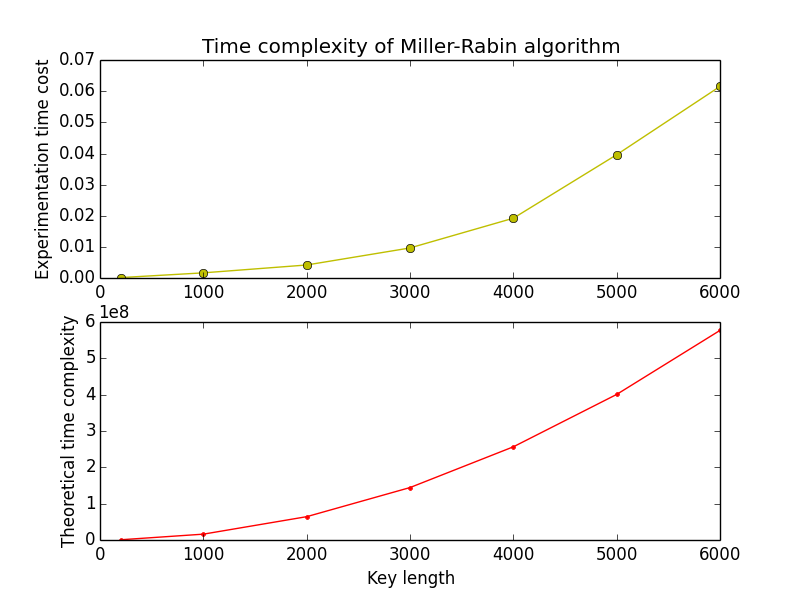
\includegraphics[scale=0.7]{rsa.png}
  \caption[]{Theoretical Time complexity vs experimentation time cost of Miller-Rabin algorithm}
  \label{fig:rsa}
\end{figure}

\chapter{\textbf{CONCLUSION}}
RSA is one of the first practical public-key cryptosystem that is widely used for secure data transmission. It must be computationally easy to encrypt and decrypt message, and computationally infeasible to determine the private key either from public key or ciphertext. The security of RSA cryptosystem bases on the length of key. Back to the question, what key length is appropriate, 200 bits, 1000 bits or more? The answer is that it depends on how fast the machine is and how efficient the algorithm is. The paper uses some efficient algorithms to implement RSA cryptosystem. From the results of chapter IV we can see that key length between 2000 and 4000 is possible to be used in practical. Since usually the RSA keys are used to encrypt symmetric keys, it's allowed to have few seconds to encrypt or decrypt data. Different from symmetric keys, which might change frequently, the RSA key pair would not change within a short period of time. As a result, the key generation is also alowed to perform several seconds. In other words, key length between 2000 bits and 4000 bits is considered to be suitable for the security at the time this paper was written.\par
In practical, the implementation of RSA usually involved in two primality test, this will significantly increase the possibility of prime number. In the future, we will analysis the time complexity of other primality tests, and compare the difference between those algorithms.
     




	
\bibliographystyle{myplain}
\clearpage
\markboth{}{}
\addcontentsline{toc}{chapter}{BIBLIOGRAPHY}
\bibliography{references}


\end{document}
